\documentclass[a4paper,12pt,oneside]{book}
\usepackage[utf8]{inputenc}
\renewcommand{\chaptername}{Part}

\usepackage{rachwidgets}

\titleformat{\chapter}[display]
  {\bfseries\Large}
  {\filright\MakeUppercase{\chaptertitlename} \Huge\thechapter}
  {1ex}
  {\titlerule\vspace{1ex}\filleft}
  [\vspace{1ex}\titlerule]

\newcommand{\laClass}       {CS 250}
\newcommand{\laSemester}    {Spring 2018}
\newcommand{\laChapter}     {}
\newcommand{\laType}        {Project}
\newcommand{\laAssignment}  {1}
\newcommand{\laPoints}      {5}
\newcommand{\laTitle}       {Unit Tests and Linear Structures}
\newcommand{\laStarterFiles}{Download from GitHub.}
\newcommand{\laTopics}      {Design, testing, UML, unit tests}
\setcounter{chapter}{1}
\setcounter{section}{1}
\addtocounter{section}{-1}
\newcounter{question}
\toggletrue{answerkey}
\togglefalse{answerkey}

\title{}
\author{Rachel Singh}
\date{\today}

\pagestyle{fancy}
\fancyhf{}

\lhead{\laClass, \laSemester}

\chead{}

\rhead{\laType\ \laAssignment: \laTitle\ \iftoggle{answerkey}{ KEY }{}}

\rfoot{\thepage\ of \pageref{LastPage}}

\lfoot{\scriptsize By Rachel Singh, last updated \today}

\renewcommand{\headrulewidth}{2pt}
\renewcommand{\footrulewidth}{1pt}

\begin{document}




\footnotesize
~\\ 
\textbf{\laType\ \laAssignment: \laTitle \tab } 
Homework projects should be worked on by each individual student.
Brainstorming and sketching out problems on paper or on a whiteboard
together are permitted, but \underline{do not} copy code from someone else
or allow your code to be copied. Students who commit or aid in plagiarism will
receive a 0\% on the assignment and be reported.

\hrulefill
\normalsize 

    \subsection*{Information}
    
        \paragraph{Topics:} \laTopics

        \paragraph{Turn in:}
            Turn in all source files - .cpp, .hpp, and/or .h files.
            \textbf{Do not turn in Visual Studio files}.

        \paragraph{Starter files:} \laStarterFiles

        \paragraph{Building and running:} If you are using Visual Studio,
            make sure to run \underline{with} debugging. (Don't run without debugging!)
            Using the debugger will help you find errors. \\
            To prevent a program exit, use this before \texttt{return 0;}
\begin{verbatim}
cin.ignore();
cin.get();
\end{verbatim}

        \paragraph{Tips:}
            \begin{itemize}
                \item   \underline{Always make sure it builds.}
                        Only add a few lines of code at a time and build
                        after each small change to ensure your program still builds.
                        
                \item   \underline{One feature at a time.}
                        Only implement one feature (or one function) at a time.
                        Make sure it builds, runs, and works as intended before
                        moving on to the next feature.
                        
                \item   \underline{Search for build errors.}
                        Chances are someone else has had the same build error before.
                        Copy the message into a search engine and look for information
                        on \textit{why} it occurs, and \textit{how} to resolve it.

                \item   \underline{Use debug tools,} such as breakpoints,
                        stack trace, and variable watch.
                
                \item   \underline{Don't implement everything in one go.}
                        Don't just try typing out all the code in one go
                        without building, running, and testing. It will be
                        much harder to debug if you've tried to program everything all at once.
            \end{itemize}

        \tableofcontents

    \newpage


    \section{About}

    Linear data structures may be implemented in different ways behind-the-scenes,
    but the general functionality should still result in the same outcome.
    For this project, you will design and implement unit tests for a linear structure,
    and these tests will be tested against the Bag data type, a smart Dynamic Array,
    and eventually the Linked List object.

    \subsection{Test files}

    In the starter code, there are the following files:

    \begin{itemize}
        \item   \texttt{tester\_program.cpp} - contains \texttt{main()}
        \item   \texttt{Tester.hpp} - the class and function declarations
        \item   \texttt{Tester.cpp} - the tester function definitions
        \item   \texttt{List.hpp} - A List class, with stub functions
    \end{itemize}

    The List class will have placeholders in the methods so that the program
    will be buildable. You will remove the placeholders as the functions are
    being implemented.

    Before implementing the functions, your first task is to implement the tests.
    As you implement the tests, they will start of failing (for the most part),
    which is good. Then, when you implement the actual functionality, you can
    validate that it works as intended by whether it passes the tests.

    Your tests may not be correct at first since this might be a new concept,
    so in some cases it is okay to adjust your tests. You might also have to
    add additional test cases to more fully cover the functionality.

    Once these tests are implemented and working with a static array-based
    list, then the tests should also theoretically work with other linear
    structures.

    \subsection{Three turn ins}

    You will turn in this project in three parts: First, the Test Outline
    document (edit in LibreOffice or MS Word and turn in). Second, the
    test implementations in the code. Third, the full List implementation.

    \newpage

    \section{Part 1 - Planning Tests}

    Make sure you download the \textbf{Test Outline} document. This is
    a document you can open up in MS Word or LibreOffice. Work on
    planning your test sets during class. You can also brainstorm
    with other students on this part.

    ~\\ Your tests should, at minimum, cover all reasonable outputs.
    For example, for something that returns a \texttt{boolean},
    we should have tests that expect a true and a false as outputs.
    For a function that returns an \texttt{integer}, such as \texttt{Size()},
    you won't test all possible outputs, but at least for 0, 1, and
    several other values.

    \begin{figure}[h]
        \centering
        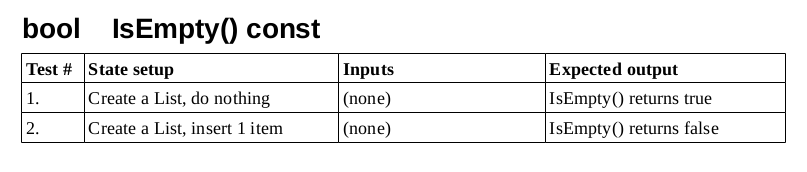
\includegraphics[width=14cm]{images-2018-01/example-test.png}
        \caption{An example of tests for the IsEmpty() function, in the Test Outline document.}
    \end{figure}

    We will work on this part during class, and for Part 1 of the project
    you can brainstorm and collaborate with other students. However,
    keep in mind that your code in Part 2 and Part 3 should be your own.

    \newpage
    
    \section{Part 2 - Writing Tests}

    \color{red} For this part of the project you should be working just on the tests,
    not the List functions. \color{black}
    You will upload this project in two parts: Just the tests, and then the
    tests with the List code.

    Reference the \textbf{Function Specifications} section for descriptions of the functions

    \subsection{Writing unit tests}

    Each unit test is meant to test one function each, though you might have to rely on
    multiple functions to fully validate a function. For example, to test the \texttt{Size()}
    function, you need to be able to add new items to the list, so \texttt{Push(...)} will have
    to be implemented for the \texttt{Size()} test to work properly.

    ~\\ Each test function may need multiple tests to properly coverage all reasonable
    use cases.

    ~\\ For each test, you will need to decide on \textbf{inputs} to pass in,
    and the \textbf{expected output}. To get the \textbf{actual output}, you will
    call the function being tested, and store its return value in a variable.

    ~\\ You can use an if statement to check whether the actual output matches
    the expected output. If they match, the individual test can \textit{pass}.
    If they don't match, the test \textit{fails}.

    ~\\ It's up to you for what to output to the screen, though generally it helps
    if you output the inputs and outputs, and whether the test passes or fails.

    \subsection{Tests to implement}

    The tests to implement are:

    \begin{center}
        \begin{tabular}{p{4cm} p{4cm} p{4cm} }
        Test\_Init() &
        Test\_ShiftRight() &
        Test\_ShiftLeft()
        \\
        Test\_Size() &
        Test\_IsEmpty() &
        Test\_IsFull()
        \\
        Test\_PushFront() &
        Test\_PushBack() &
        Test\_PopFront()
        \\
        Test\_PopBack() &
        Test\_Clear() &
        Test\_Get()
        \\
        Test\_GetFront() &
        Test\_GetBack() &
        Test\_GetCountOf()
        \\
        Test\_Contains() &
        Test\_Remove() &
        Test\_Insert()
        \end{tabular}
    \end{center}

\subsection{Example test:}

\begin{lstlisting}[style=code]
void Tester::Test_Size()
{
    DrawLine();
    cout << "TEST: Test_Size" << endl;

    {   // Test begin
        cout << "\n \n Test 1";
        List<int> testList;
        int expectedSize = 0;
        int actualSize = testList.Size();

        cout << "\n Expected size: " << expectedSize;
        cout << "\n Actual size:   " << actualSize;

        if ( actualSize == expectedSize )
            cout << "\n Pass";
        else
            cout << "\n Fail";
    }   // Test end

    {   // Test begin
        cout << endl << "Test 2" << endl;
        List<int> testList;

        testList.PushBack( 1 );
        testList.PushBack( 3 );

        int expectedSize = 2;
        int actualSize = testList.Size();

        cout << "\n Expected size: " << expectedSize;
        cout << "\n Actual size:   " << actualSize;

        if ( actualSize == expectedSize )
            cout << "\n Pass";
        else
            cout << "\n Fail";
    }   // Test end
}
\end{lstlisting}

    \subsection{Example output:}

    An example of a couple of tests failing, since the List functions haven't
    been implemented yet.
    
\begin{lstlisting}[style=output]
----------------------------------------------------------------------------
TEST: Test_Size

Test 1
Expected size: 0
Actual size:   -1585510992
Fail

Test 2
Expected size: 1
Actual size:   -1585510992
Fail
\end{lstlisting}

    \hrulefill

    \section{Part 3 - Implementing the List}

    Once you've implemented the tests, you will be implementing the
    List functions based on the functionality specified. As you
    get each function working, your tests should be passing.

    Note that certain tests may rely on the implementation of other
    functions, such as \texttt{Size()} needing a Push function implemented
    in order to test for more cases than just an empty list.

    \newpage

    \section{Function Specifications}

    \begin{figure}[h]
        \centering
        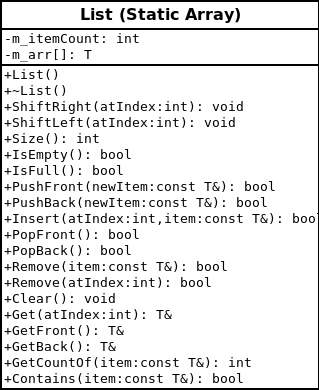
\includegraphics[height=8cm]{images-2018-01/List.png}
        \caption{A List class UML diagram, implemented with a static array}
    \end{figure}

    % ---------------------------------------------------------------- %
    \begin{framed}
    \subsection{IsEmpty}

    Function header: \texttt{bool    IsEmpty() const}

    \paragraph{Inputs:}
        None

    \paragraph{Outputs:}
        \texttt{true} if there is nothing in the list (i.e., the size is 0), or \texttt{false} if not.

    \end{framed}

    \newpage

    % ---------------------------------------------------------------- %
    \begin{framed}
    \subsection{IsFull}

    Function header: \texttt{bool    IsFull() const}

    \paragraph{Inputs:}
        None

    \paragraph{Outputs:}
        \texttt{true} if the list is full (i.e., the \texttt{m\_itemCount} is equal to \texttt{ARRAY\_SIZE}),
        or \texttt{false} if not.
        
    \end{framed}

    % ---------------------------------------------------------------- %
    \begin{framed}
    \subsection{Size}

    Function header: \texttt{int     Size() const}

    \paragraph{Inputs:}
        None

    \paragraph{Outputs:}
        Returns the amount of items stored in the list. Will be $\geq 0$.

    \end{framed}

    %\newpage
    
    % ---------------------------------------------------------------- %
    \begin{framed}
    \subsection{GetCountOf}

    Function header: \texttt{int     GetCountOf( const T\& item ) const}

    \paragraph{Inputs:}
        \texttt{const T\& item}, where the list contains items of type \texttt{T} (it is a template).
        The item to be searched for and counted is \texttt{item}.

    \paragraph{Outputs:}
        Returns the amount of instances of \texttt{item} being found in the list.
        Will be $\geq 0$.

    \end{framed}

    \newpage
    
    % ---------------------------------------------------------------- %
    \begin{framed}
    \subsection{Contains}

    Function header: \texttt{bool    Contains( const T\& item ) const}

    \paragraph{Inputs:}
        \texttt{const T\& item}, where \texttt{item} is the item to search for.

    \paragraph{Outputs:}
        Returns \texttt{true} if \texttt{item} is found in the list, and \texttt{false} otherwise.

    \end{framed}
    
    % ---------------------------------------------------------------- %
    \begin{framed}
    \subsection{List constructor}

    Function header: \texttt{List()}

    ~\\ Initializes the List class. The list should start off empty.

    \paragraph{Inputs:}
        None

    \end{framed}
    
    % ---------------------------------------------------------------- %
    \begin{framed}
    \subsection{List destructor (no tests)}

    ~\\ Nothing required for the static array version of the List.

    \end{framed}

    \newpage
    
    % ---------------------------------------------------------------- %
    \begin{framed}
    \subsection{PushFront}

    Function header: \texttt{bool    PushFront( const T\& newItem )}

    \paragraph{Inputs:}
        \texttt{const T\& item}, the new item to add to the list at the beginning.

    \paragraph{Outputs:}
        Returns \texttt{true} if the operation is a success, and \texttt{false} otherwise.

    \end{framed}
    
    % ---------------------------------------------------------------- %
    \begin{framed}
    \subsection{PushBack}

    Function header: \texttt{bool    PushBack( const T\& newItem )}

    \paragraph{Inputs:}
        \texttt{const T\& item}, the new item to add to the list at the end.

    \paragraph{Outputs:}
        Returns \texttt{true} if the operation is a success, and \texttt{false} otherwise.

    \end{framed}
    
    % ---------------------------------------------------------------- %
    \begin{framed}
    \subsection{Insert}

    Function header: \texttt{bool    Insert( int atIndex, const T\& item )}

    ~\\ Inserts a new item at the given index. Existing items shouldn't
    be replaced. If there is an item already at the index given, it will be
    pushed towards the end of the list.

    \paragraph{Inputs:}
        \begin{itemize}
            \item   \texttt{int atIndex} - the index where to insert the new item.
            \item   \texttt{const T\& item} - the new item to insert.
        \end{itemize}

    \paragraph{Outputs:}
        Returns \texttt{true} if the operation is a success, and \texttt{false} otherwise.

    \end{framed}

    \newpage
    
    % ---------------------------------------------------------------- %
    \begin{framed}
    \subsection{Get}

    Function header: \texttt{T*      Get( int atIndex )}

    \paragraph{Inputs:}
        \texttt{int atIndex}, the index of the item to return.

    \paragraph{Outputs:}
        Returns the address of the item at the index given, or \texttt{nullptr} if it isn't found.

    \end{framed}
    
    % ---------------------------------------------------------------- %
    \begin{framed}
    \subsection{GetFront}

    Function header: \texttt{T*      GetFront()}

    \paragraph{Inputs:}
        None

    \paragraph{Outputs:}
        Returns the address of the item at the front of the list, or \texttt{nullptr} if the list is empty.

    \end{framed}
    
    % ---------------------------------------------------------------- %
    \begin{framed}
    \subsection{GetBack}

    Function header: \texttt{T*      GetBack()}

    \paragraph{Inputs:}
        None

    \paragraph{Outputs:}
        Returns the address of the item at the end of the list, or \texttt{nullptr} if the list is empty.

    \end{framed}

    \newpage
    
    % ---------------------------------------------------------------- %
    \begin{framed}
    \subsection{PopFront}

    Function header: \texttt{bool    PopFront()}

    \paragraph{Inputs:}
        None

    \paragraph{Outputs:}
        Returns \texttt{true} if removing the item is successful, and \texttt{false} otherwise.

    \end{framed}
    
    % ---------------------------------------------------------------- %
    \begin{framed}
    \subsection{PopBack}

    Function header: \texttt{bool    PopBack()}

    \paragraph{Inputs:}
        None

    \paragraph{Outputs:}
        Returns \texttt{true} if removing the item is successful, and \texttt{false} otherwise.

    \end{framed}
    
    % ---------------------------------------------------------------- %
    \begin{framed}
    \subsection{Remove}

    Function header: \texttt{bool    Remove( const T\& item )}
    Function header: \texttt{bool    Remove( int atIndex )}

    \paragraph{Inputs:}
        \begin{itemize}
            \item   \texttt{const T\& item} - locates all instances of this item in the list and removes it.
            \item   \texttt{int atIndex} - removes the item at this index.
        \end{itemize}

    \paragraph{Outputs:}
        Returns \texttt{true} if removing the item is successful, and \texttt{false} otherwise.

    \end{framed}
    
    % ---------------------------------------------------------------- %
    \begin{framed}
    \subsection{Clear}

    Function header: \texttt{void    Clear()}

    ~\\ Clears out the list. To test this function, you should ensure that
    the size of the list returns to 0 after this function is called.

    \paragraph{Inputs:}
        None

    \paragraph{Outputs:}
        None

    \end{framed}
    
    % ---------------------------------------------------------------- %
    \begin{framed}
    \subsection{ShiftRight}

    Function header: \texttt{bool ShiftRight( int atIndex )}

    ~\\ Moves everything to the right of the index further to the right by one position.

    \paragraph{Inputs:}
        \texttt{int atIndex} - The index at which to begin moving items forward.

    \paragraph{Outputs:}
        Returns \texttt{true} if the shift is successful, or \texttt{false} if not.

    \end{framed}
    
    % ---------------------------------------------------------------- %
    \begin{framed}
    \subsection{ShiftLeft}

    Function header: \texttt{bool ShiftLeft( int atIndex )}

    ~\\ Moves everything to the right of the index further to the left by one position.
    This will overwrite the item at the \texttt{atIndex}.

    \paragraph{Inputs:}
        None

    \paragraph{Outputs:}
        Returns \texttt{true} if the shift is successful, or \texttt{false} if not.

    \end{framed}

    
    % ---------------------------------------------------------------- %
    % ---------------------------------------------------------------- %
    % ---------------------------------------------------------------- %

    \section{Grading breakdown}

    \begin{figure}[h]
        \centering
        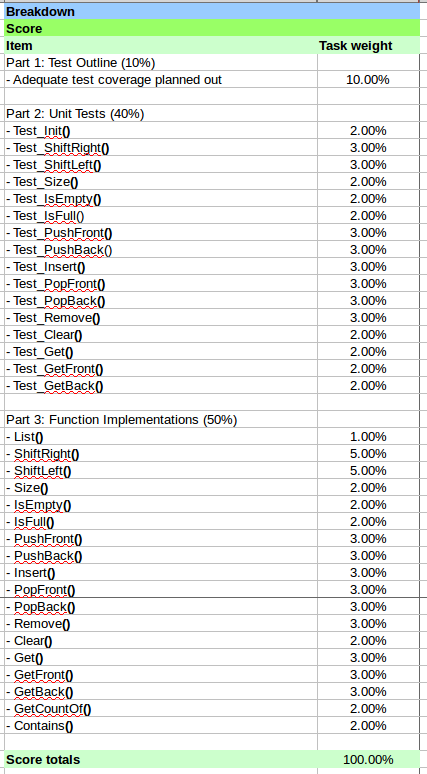
\includegraphics[height=16cm]{images-2018-01/2018-01-project1-breakdown1.png}
    \end{figure}

    \begin{figure}[h]
        \centering
        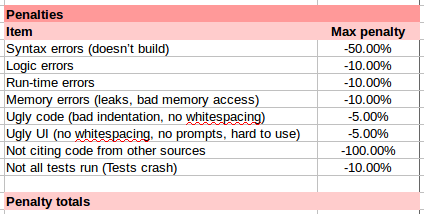
\includegraphics{images-2018-01/2018-01-project1-breakdown2.png}
    \end{figure}
    


\end{document}

